%%%%%%%%%%%%%%%%%%%%%%%%%%%%%%%%%%%%%
%                                   %
% Compile with XeLaTeX and biber    %
%                                   %
% Questions or comments:            %
%                                   %
% joshua dot mcneill at uga dot edu %
%                                   %
%%%%%%%%%%%%%%%%%%%%%%%%%%%%%%%%%%%%%

\documentclass{beamer}
  % Read in standard preamble (cosmetic stuff)
  %%%%%%%%%%%%%%%%%%%%%%%%%%%%%%%%%%%%%%%%%%%%%%%%%%%%%%%%%%%%%%%%
% This is a standard preamble used in for all slide documents. %
% It basically contains cosmetic settings.                     %
%                                                              %
% Joshua McNeill                                               %
% joshua dot mcneill at uga dot edu                            %
%%%%%%%%%%%%%%%%%%%%%%%%%%%%%%%%%%%%%%%%%%%%%%%%%%%%%%%%%%%%%%%%

% Beamer settings
% \usetheme{Berkeley}
\usetheme{CambridgeUS}
% \usecolortheme{dove}
% \usecolortheme{rose}
\usecolortheme{seagull}
\usefonttheme{professionalfonts}
\usefonttheme{serif}
\setbeamertemplate{bibliography item}{}

% Packages and settings
\usepackage{fontspec}
  \setmainfont{Charis SIL}
\usepackage{hyperref}
  \hypersetup{colorlinks=true,
              allcolors=blue}
\usepackage{graphicx}
  \graphicspath{{../../figures/}}
\usepackage[normalem]{ulem}
\usepackage{enumerate}

% Document information
\author{M. McNeill}
\title[FREN2001]{Français 2001}
\institute{\url{joshua.mcneill@uga.edu}}
\date{}

%% Custom commands
% Lexical items
\newcommand{\lexi}[1]{\textit{#1}}
% Gloss
\newcommand{\gloss}[1]{`#1'}
\newcommand{\tinygloss}[1]{{\tiny`#1'}}
% Orthographic representations
\newcommand{\orth}[1]{$\langle$#1$\rangle$}
% Utterances (pragmatics)
\newcommand{\uttr}[1]{`#1'}
% Sentences (pragmatics)
\newcommand{\sent}[1]{\textit{#1}}
% Base dir for definitions
\newcommand{\defs}{../definitions}


  % Packages and settings
  \usepackage{adjustbox}
  \usepackage[backend=biber, style=apa]{biblatex}
    \addbibresource{../References.bib}

  % Document information
  \subtitle[Consonant Articulation]{Articulation of English Consonants}

  %% Custom commands
  % Subsection/frame titles
  \newcommand{\suboneone}{Definition}
  \newcommand{\subonetwo}{Three questions}
  \newcommand{\subtwoone}{Components and mechanisms}
  \newcommand{\subtwotwo}{Voicing}
  \newcommand{\subtwothree}{Places of articulation}
  \newcommand{\subtwofour}{Manners of articulation}
  \newcommand{\subtwofive}{Resources and practice}

\begin{document}
  % Read in the standard intro slides (title page and table of contents)
  %%%%%%%%%%%%%%%%%%%%%%%%%%%%%%%%%%%%%%%%%%%%%%%%%%%%%%%%%%%%%%%%
% This is a standard set of intro slides used in for all slide %
% documents. It basically contains the title page and table of %
% contents.                                                    %
%                                                              %
% Joshua McNeill                                               %
% joshua dot mcneill at uga dot edu                            %
%%%%%%%%%%%%%%%%%%%%%%%%%%%%%%%%%%%%%%%%%%%%%%%%%%%%%%%%%%%%%%%%

\begin{frame}
  \titlepage
  \tiny{Office: % Basically a variable for office hours location
Gilbert 121\\
        Office hours: % Basically a variable for office hours
 lundi, mercredi, vendredi 10:10--11:10
}
\end{frame}

\begin{frame}
  \tableofcontents[hideallsubsections]
\end{frame}

\AtBeginSection[]{
  \begin{frame}
    \tableofcontents[currentsection,
                     hideallsubsections]
  \end{frame}
}


  \section{What is articulatory phonetics?}
    \subsection{\suboneone}
      \begin{frame}{\suboneone}
        \begin{block}{}
          The three broad areas of phonetics:
          \begin{itemize}
            \item \alert<2->{Articulatory phonetics}
            \item Acoustic phonetics
            \item Auditory phonetics
          \end{itemize}
        \end{block}
        \begin{definition}<3>
          % Read in the definition of articulatory phonetics
          % Articulatory phonetics
The study of the physiological production of speech sounds
 (i.e., \alert{articulation})
        \end{definition}
      \end{frame}

    \subsection{\subonetwo}
      \begin{frame}{\subonetwo}
        \begin{block}{}
          Any consonant can be described by answering:
          \begin{itemize}
            \item If it is \alert{voiced} or \alert{voiceless},
            \item % Place of articulation
\emph{Where} the airstream is constricted
 (i.e., the \alert{place of articulation}), and
            \item % Manner of articulation
\emph{How} the airstream is constricted
 (i.e., the \alert{manner of articulation})
          \end{itemize}
        \end{block}
        \begin{alertblock}<2>{}
          These are called \alert{segmental features}
        \end{alertblock}
      \end{frame}

  \section{Anatomy and articulation}
    \subsection{\subtwoone}
      \begin{frame}{\subtwoone}
        \begin{columns}
          \column{0.45\textwidth}
            \only<1-2>{
              \begin{minipage}[c][0.6\textheight]{\linewidth}
                \begin{block}{Broad components}
                  \begin{itemize}
                    \only<1>{
                    \item \alert{Subglottal system}
                    \begin{itemize}
                      \item % Subglottal system
The anatomical component that controls airflow

                    \end{itemize}
                    \item \alert{Larynx}
                    \begin{itemize}
                      \item % Larynx
The anatomical component that controls voicing (and is sometimes a place of articulation)

                    \end{itemize}
                    }
                    \only<2>{
                    \item \alert{Vocal tract}
                    \begin{itemize}
                      \item % Vocal tract
The anatomical component that controls manner of articulation and contains places of articulation

                    \end{itemize}
                    }
                  \end{itemize}
                \end{block}
              \end{minipage}
            }
            \only<3>{
              \begin{minipage}[c][0.6\textheight]{\linewidth}
                \begin{block}{Sublglottal system}
                  One \alert{airstream mechanism} in English (i.e., source and direction of airflow):
                  \begin{itemize}
                    \item \alert{Pulmonic}: Lungs are the source
                    \item \alert{Egressive}: Out is the direction
                  \end{itemize}
                \end{block}
              \end{minipage}
            }
          \column{0.55\textwidth}
            \begin{block}{}
              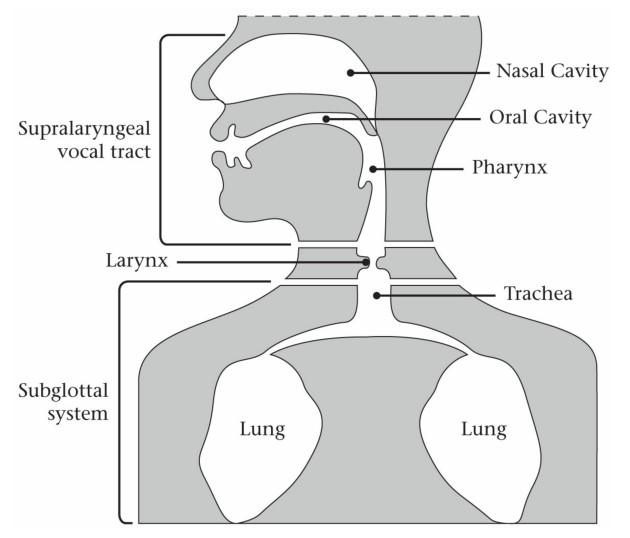
\includegraphics[scale=0.5]{anat_overall.jpg}
            \end{block}
        \end{columns}
      \end{frame}

    \subsection{\subtwotwo}
      \begin{frame}{\subtwotwo}
        \begin{columns}
          \column{0.45\textwidth}
            \only<1>{
              \begin{minipage}[c][0.6\textheight]{\linewidth}
                \begin{block}{}
                  \begin{itemize}
                    \item \alert{Voiced} sounds: % Voiced sounds
Sounds produced by vibrating the vocal folds

                    \item \alert{Voiceless} sounds: % Voiceless sounds
Sounds produced with the vocal folds wide open

                  \end{itemize}
                \end{block}
              \end{minipage}
            }
            \only<2->{
              \begin{minipage}[c][0.6\textheight]{\linewidth}
                \begin{example}
                  \begin{itemize}
                    \item \lexi{\alert{f}at} and \lexi{\alert{v}at} \uncover<3->{[f] and [v]}
                    \item \lexi{\alert{p}at} and \lexi{\alert{b}at} \uncover<4->{[p] and [b]}
                    \item \lexi{\alert{th}y} and \lexi{\alert{th}igh} \uncover<5->{[ð] and [θ]}
                    \item \lexi{\alert{z}ip} and \lexi{\alert{s}ip} \uncover<6->{[z] and [s]}
                  \end{itemize}
                \end{example}
              \end{minipage}
            }
          \column{0.55\textwidth}
            \begin{block}{Larynx}
              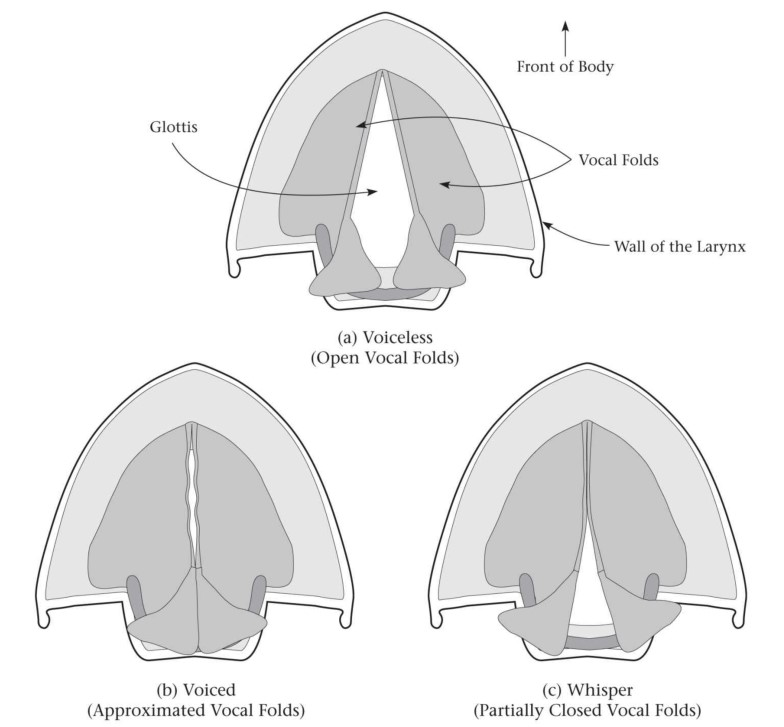
\includegraphics[scale=0.4]{anat_folds.jpg}
            \end{block}
        \end{columns}
      \end{frame}

    \subsection{\subtwothree}
      \begin{frame}{\subtwothree}
        \begin{columns}
          \column{0.45\textwidth}
            \begin{minipage}[c][0.6\textheight]{\linewidth}
              \only<1-2>{
                \begin{definition}
                  % Place of articulation
\emph{Where} the airstream is constricted
 in the vocal tract\uncover<2>{\emph{, which means we're not talking about vowels}}
                \end{definition}
              }
              \only<3>{
                \begin{alertblock}{Bilabials}
                  Constriction occurs at the lips
                \end{alertblock}
              }
              \only<4>{
                \begin{alertblock}{Labiodentals}
                  Constriction occurs between the lower lip and the upper front teeth
                \end{alertblock}
              }
              \only<5>{
                \begin{alertblock}{Interdentals}
                  Constriction occurs by placing the tip of the tongue between the teeth
                \end{alertblock}
              }
              \only<6>{
                \begin{alertblock}{Alveolars}
                  Constriction occurs by placing the tip of the tongue against the alveolar ridge
                \end{alertblock}
              }
              \only<3-6>{
                \begin{example}
                  \begin{itemize}
                    \item \lexi{\alert{f}at} and \lexi{\alert{v}at} [f] and [v]
                    \item \lexi{\alert{p}at} and \lexi{\alert{b}at} [p] and [b]
                    \item \lexi{\alert{th}y} and \lexi{\alert{th}igh} [ð] and [θ]
                    \item \lexi{\alert{z}ip} and \lexi{\alert{s}ip} [z] and [s]
                  \end{itemize}
                \end{example}
              }
              \only<7-9>{
                \begin{alertblock}{Post-alveolars}
                  Constriction occurs by placing the tip of the tongue against the area between the alveolar ridge and the hard palate
                \end{alertblock}
                \begin{example}<8-9>
                  \lexi{delu\alert{s}ion} and \lexi{dilu\alert{t}ion} \uncover<9>{[ʒ] and [ʃ]}
                \end{example}
              }
              \only<10-11>{
                \begin{alertblock}{Palatals}
                  Constriction occurs by placing the body of the tongue against the hard palate
                \end{alertblock}
                \begin{example}<11>
                  \lexi{\alert{y}es} [j]
                \end{example}
              }
              \only<12-14>{
                \begin{alertblock}{Velars}
                  Constriction occurs by placing the back of the tongue against the velum/soft palate
                \end{alertblock}
                \begin{example}<13-14>
                  \lexi{\alert{k}ill} and \lexi{\alert{g}ill} \uncover<14>{[k] and [g]}
                \end{example}
              }
              \only<15-16>{
                \begin{alertblock}{Glottals}
                  Constriction occurs in the larynx
                \end{alertblock}
                \begin{example}<16>
                  \lexi{\alert{h}igh} and \lexi{co\alert{tt}on} {[h] and [ʔ]}
                \end{example}
              }
            \end{minipage}
          \column{0.55\textwidth}
            \begin{block}{Vocal tract}
              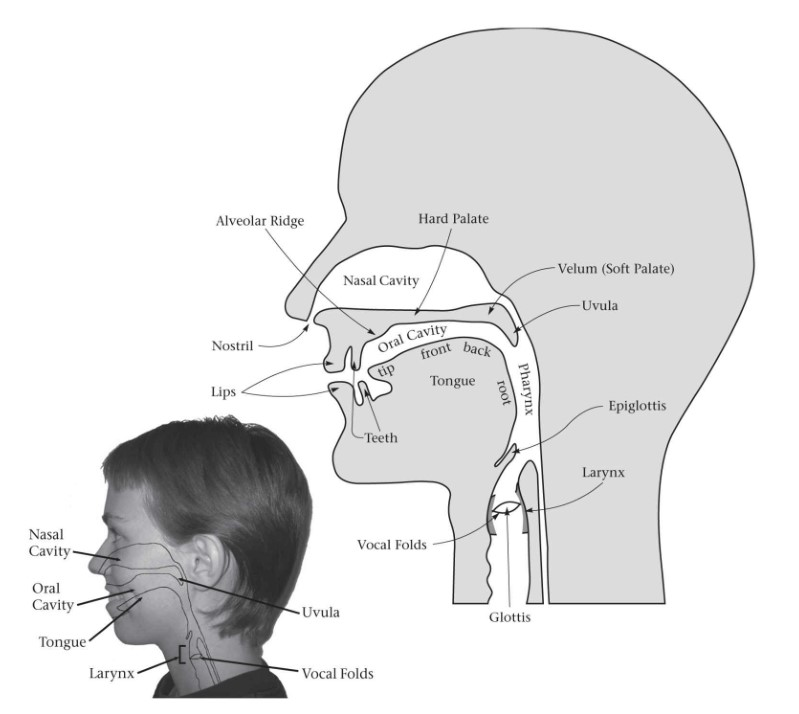
\includegraphics[scale=0.4]{anat_places.jpg}
            \end{block}
        \end{columns}
      \end{frame}

    \subsection{\subtwofour}
      \begin{frame}[t]{\subtwofour}
        \only<1-2>{
          \begin{definition}
            % Manner of articulation
\emph{How} the airstream is constricted
 in the vocal tract\uncover<2>{, \emph{which means we're still talking about consonants}}
          \end{definition}
        }
        \only<3->{
          \begin{block}{Sonority hierarchy}
            stops/plosives $\rightarrow$ affricates $\rightarrow$ fricatives $\rightarrow$ nasals $\rightarrow$ flaps $\rightarrow$ approximants (liquids $\rightarrow$ glides)
          \end{block}
        }
        \only<4-6>{
          \begin{alertblock}{Stops/plosives}
            Constriction of the airstream is complete, and the sound is generated by the release of that constriction
          \end{alertblock}
          \begin{example}<5-6>
            \begin{itemize}
              \item \lexi{\alert{p}at} and \lexi{\alert{b}at} [p] and [b], as well as \lexi{co\alert{tt}on} [ʔ]
              \item<6> voiceless bilabial, voiced bilabial, glottal
            \end{itemize}
          \end{example}
        }
        \only<7-13>{
          \begin{alertblock}{Fricatives}
            Constriction of the airstream is \emph{nearly} complete, causing turbulence and creating a hissing sound
          \end{alertblock}
          \begin{example}<8-13>
            \only<8-9>{
              \begin{itemize}
                \item \lexi{\alert{f}at} and \lexi{\alert{v}at} [f] and [v]
                \item<9> voiceless labiodental, voiced labiodental
              \end{itemize}
            }
            \only<10-11>{
              \begin{itemize}
                \item \lexi{\alert{th}y} and \lexi{\alert{th}igh} [ð] and [θ]
                \item<11> voiced interdental, voiceless interdental
              \end{itemize}
            }
            \only<12-13>{
              \begin{itemize}
                \item \lexi{\alert{z}ip} and \lexi{\alert{s}ip} [z] and [s]
                \item<13> voiced alveolar, voiceless aveolar
              \end{itemize}
            }
          \end{example}
        }
        \only<14-16>{
          \begin{alertblock}{Affricates}
            Constriction of the airstream is the combination of a stop followed by a fricative
          \end{alertblock}
          \begin{example}<15-16>
            \begin{itemize}
              \item \lexi{\alert{j}u\alert{dg}e} and \lexi{church} [dʒ] and [tʃ]
              \item<16> voiced post-alveolar, voiceless post-alveolar
            \end{itemize}
          \end{example}
        }
        \only<17-19>{
          \begin{alertblock}{Nasals}
            Constriction of the airstream is created by lowering the velum in combination with a stop articulation, thus directing the airstream through the nasal cavity
          \end{alertblock}
          \begin{example}<18-19>
            \begin{itemize}
              \item \lexi{Ki\alert{m}}, \lexi{ki\alert{n}}, and \lexi{ki\alert{ng}} [m], [n], and [ŋ]
              \item<19> voiced bilabial, voiced alveolar, voiced velar
            \end{itemize}
          \end{example}
        }
        \only<20-22>{
          \begin{alertblock}{Flaps}
            Constriction of the airstream is complete \emph{but very rapid}
          \end{alertblock}
          \begin{example}<21-22>
            \begin{itemize}
              \item \lexi{toma\alert{t}o} and \lexi{wri\alert{t}er} [ɾ]
              \item<22> alveolar
            \end{itemize}
          \end{example}
        }
        \only<23>{
          \begin{alertblock}{Approximants}
            Constriction of the airstream is less complete than for fricatives, lacking the turbulence that creates the hissing sound
            \begin{itemize}
              \item Two types: liquids and glides
            \end{itemize}
          \end{alertblock}
        }
        \only<24-27>{
          \begin{alertblock}{Liquids}
            Constriction of the airstream is less than for fricatives, and there is no movement involved in the articulation
          \end{alertblock}
          \begin{example}<25-27>
            \begin{itemize}
              \item \lexi{\alert{r}ead} and \lexi{tab\alert{l}e} [ɹ] and [l̩]
              \item<26-27> voiced alveolar, voiced lateral alveolar
              \item<27> {[}ɹ{]} is sometimes retroflex
            \end{itemize}
          \end{example}
        }
        \only<28-30>{
          \begin{alertblock}{Glides}
            Constriction of the airstream is less than for fricatives, and there \emph{is} movement involved in the articulation
          \end{alertblock}
          \begin{example}<29-30>
            \begin{itemize}
              \item \lexi{\alert{wh}ich} and \lexi{\alert{yawn}} [w] and [j]
              \item<30> voiced labial-velar, voiced palatal
            \end{itemize}
          \end{example}
        }
      \end{frame}

    \subsection{\subtwofive}
      \begin{frame}{\subtwofive}
        \begin{block}{}
          \begin{itemize}
            \item To hear these sounds: \url{http://web.uvic.ca/ling/resources/ipa/charts/IPAlab/IPAlab.htm}
            \item To type these symbols: \url{https://ipa.typeit.org/}
          \end{itemize}
        \end{block}
        \begin{adjustbox}{width=\textwidth}
          % Read in English IPA consonant chart
          %%%%%%%%%%%%%%%%%%%%%%%%%%%%%%%%%%%%%%%%%%%%%%%%%%%%%%%%%%
% This creates an English IPA chart for consonants       %
%                                                        %
% Compiled from material_IPA_en_chart.tex when a         %
% standalone document is needed                          %
%                                                        %
% -Joshua McNeill (joshua dot mcneill at uga dot edu)    %
%%%%%%%%%%%%%%%%%%%%%%%%%%%%%%%%%%%%%%%%%%%%%%%%%%%%%%%%%%

\begin{tabular}{| l | c c | c c | c c | c c | c c | c c | c c | c c | c c | c c | c c |}
  \hline
  & \multicolumn{2}{c}{Bilabial} & \multicolumn{2}{c}{Labiodental} & \multicolumn{2}{c}{Dental} & \multicolumn{2}{c}{Alveolar} & \multicolumn{2}{c}{Postalveolar} & \multicolumn{2}{c}{Retroflex} & \multicolumn{2}{c}{Palatal} & \multicolumn{2}{c}{Velar} & \multicolumn{2}{c}{Uvular} & \multicolumn{2}{c}{Pharyngeal} & \multicolumn{2}{c}{Glottal} \\
  \hline
  Plosive/Stop & p & b &   &   &   &   & t & d &   &   & & & &   & k & ɡ & & & & & ʔ & \\
  \hline
  Nasal        &   & m &   &   &   &   &   & n &   &   & & & &   &   & ŋ & & & & &   & \\
  \hline
  Trill        &   &   &   &   &   &   &   &   &   &   & & & &   &   &   & & & & &   & \\
  \hline
  Tap/Flap     &   &   &   &   &   &   &   & ɾ &   &   & & & &   &   &   & & & & &   & \\
  \hline
  Fricative    &   &   & f & v & θ & ð & s & z & ʃ & ʒ & & & &   &   &   & & & & & h & \\
  \hline
  \begin{tabular}{@{} l @{}}
    Lateral \\
    fricative
  \end{tabular}&   &   &   &   &   &   &   &   &   &   & & & &   &   &   & & & & &   & \\
  \hline
  Approximant  &   &   &   &   &   &   &   & ɹ &   &   & & & & j &   &   & & & & &   & \\
  \hline
  \begin{tabular}{@{} l @{}}
    Lateral\\
    approximant
  \end{tabular}&   &   &   &   &   &   &   & l &   &   & & & &   &   &   & & & & &   & \\
  \hline
\end{tabular}

        \end{adjustbox}
        \begin{block}{Try these}
          \textcite{dawson_language_2016}, chapter 2 exercises 5, 6, 8
        \end{block}
      \end{frame}
\end{document}
